%!TEX root = ../thesis.tex
%*******************************************************************************
%******************************   Fourth Chapter   ***************************
%*******************************************************************************
\chapter{Improving \ont{} sequencing accuracy for \mtb{}}
\label{chap:tubby}
%%%%%%%%%%%%%%%%%%%%%%%%%%%%%%%%%%%%%%%%%%%%%%%%%%%%%%%%%%%%%%%%%%%%%%%%%%%%%%%%%

\setcounter{section}{-1}
\section{Publication and collaboration acknowledgements}
\label{sec:ch4-acknowledge}

%%%%%%%%%%%%%%%%%%%%%%%%%%%%%%%%%%%%%%%%%%%%%%%%%%%%%%%%%%%%%%%%%%%%%%%%%%%%%%%%%
\section{Introduction}

Taxon-specific \ont{} basecalling models have been shown to provide increased read and consensus accuracy(CITE).
It has previously been shown(CITE) that a taxon-specific basecalling model can improve both the read-level and consensus accuracy of \ont{} sequencing reads. While this was shown for *Klebsiella pneumoniae*, it remains to be seen if this approach generalises to other species.

%%%%%%%%%%%%%%%%%%%%%%%%%%%%%%%%%%%%%%%%%%%%%%%%%%%%%%%%%%%%%%%%%%%%%%%%%%%%%%%%%
\section{Dataset}
\label{sec:tubby-data}

 Perhaps the most important aspect of training a basecalling model is providing a "truth" for the data. In the context of training a \ont{} basecalling model, truth data refers to high-quality genome assemblies for the training samples. The \ont{} basecaller, \guppy{}, uses neural networks to convert the raw electrical signal into a DNA sequence. In order to train the network in how to make this inference it is necessary to label the raw signal with its corresponding "truth" sequence. Such datasets are difficult to find for certain species. However, the dataset we have collected for the work \autoref{chap:clustering} and \autoref{chap:dst} is perfectly suited. It contains samples with Illumina, PacBio, and \ont{} sequencing data from the exact same DNA extraction, ensuring any discrepancies between the \ont{} data and the truth are technology differences, and not \textit{in vitro} evolution. 

For the training and validation of our \mtb{}-specific model, we use the eight samples we generated high-quality assemblies from PacBio data in \autoref{sec:asm_results} (see \autoref{app:asm} for full methods). We use the PacBio assemblies produced by \flye{} and polished with Illumina by Pilon - not correcting for SNPs. By using the Illumina-polished PacBio assemblies for each sample we ensure no \ont{} biases are present in the truth genomes that the new model is being trained from.

In addition to the eight training and validation samples, we evaluate on a \ont{} sequencing run of the \textit{Mycobacterium bovis} strain used in the Bacille Calmette-Guérin (BCG) vaccine. This strain (AF2122/97) is an attenuated \textit{M. bovis} bacillus \cite{luca2013} with a well-characterised reference genome (accession LT708304.1) \cite{Malone2017}. As the genome similarity between \textit{M. bovis} and \mtb{} is 99.95\% \cite{Kanipe2020}, this BCG strain acts as a great test for the model's ability to call both a sample not from the training set and not from the exact species, but a very closely related one.

\todo[inline]{add BCG sequencing methods}
%  I have emailed Sophie requesting these methods

%%%%%%%%%%%%%%%%%%%%%%%%%%%%%%%%%%%%%%%%%%%%%%%%%%%%%%%%%%%%%%%%%%%%%%%%%%%%%%%%%
\section{Training an \mtb{}-specific \ont{} basecalling model}

In order to be train a basecalling model for use with \guppy{}, there are a number of preparation steps required. For many of these preparation steps, we use the open-source software, Taiyaki, developed by Oxford Nanopore Technologies (ONT) to train their RNA and DNA model for \guppy{} (\url{https://github.com/nanoporetech/taiyaki}).

We trained an \mtb{}-specific basecalling model - named \tubby{} - for use with three different versions of \guppy{}: 3.4.5, 3.6.0, and 4.4.0. The preparation, training, and evaluation steps are the same for each model, with the only difference being the version of \guppy{} used to basecall the initial data, and the pretrained models used to begin training from.

\subsubsection{Preparation}

In the first stage of preparing the data for training, we basecall and demultiplex the data with the relevant version of \guppy{} using the default high-accuracy model configurations (HAC). Next, we align the basecalled reads for each sample to their truth assembly (\autoref{sec:tubby-data}) with \vrb{minimap2} \cite{li2018}, discarding unmapped and secondary alignments.

The sequence for each aligned read is then replaced with the reference sequence it aligns to - in the same orientation - using \taiyaki{}. Any read with less than 50\%  of its sequence aligned is discarded in this process. The resulting FASTA file from this step acts as a way of mapping a read identifier to its truth sequence during training and contained 1,309,759 read-references.

The recommended number of reads for \taiyaki{} model-training is in the range of tens-of-thousands or low hundreds-of-thousands if read lengths are greater than 1000bp or less than 500bp, respectively. As our read-reference file has many more sequences than is required, we randomly sub-sampled the FASTA file into two chunks with 20\% (261,950) for training and the remainder (1,047,807) to be used for validation of the final model. Using the list of read identifiers in these two subsets, we extract the raw (fast5) data for each read into separate training and evaluation batches. 

Next, we use \taiyaki{} to trim 200 and 100 raw signal events from the start and end, respectively, of each training read. This trimming essentially serves to remove adapter and barcodes signals. \taiyaki{} is then used to align the raw signal for a read to its sequence in the read-reference file. This mapping is a vital preparation step that creates a signal-to-sequence file indicating what nucleotides are associated with a given collection of the raw signals and vice versa.

\begin{figure}
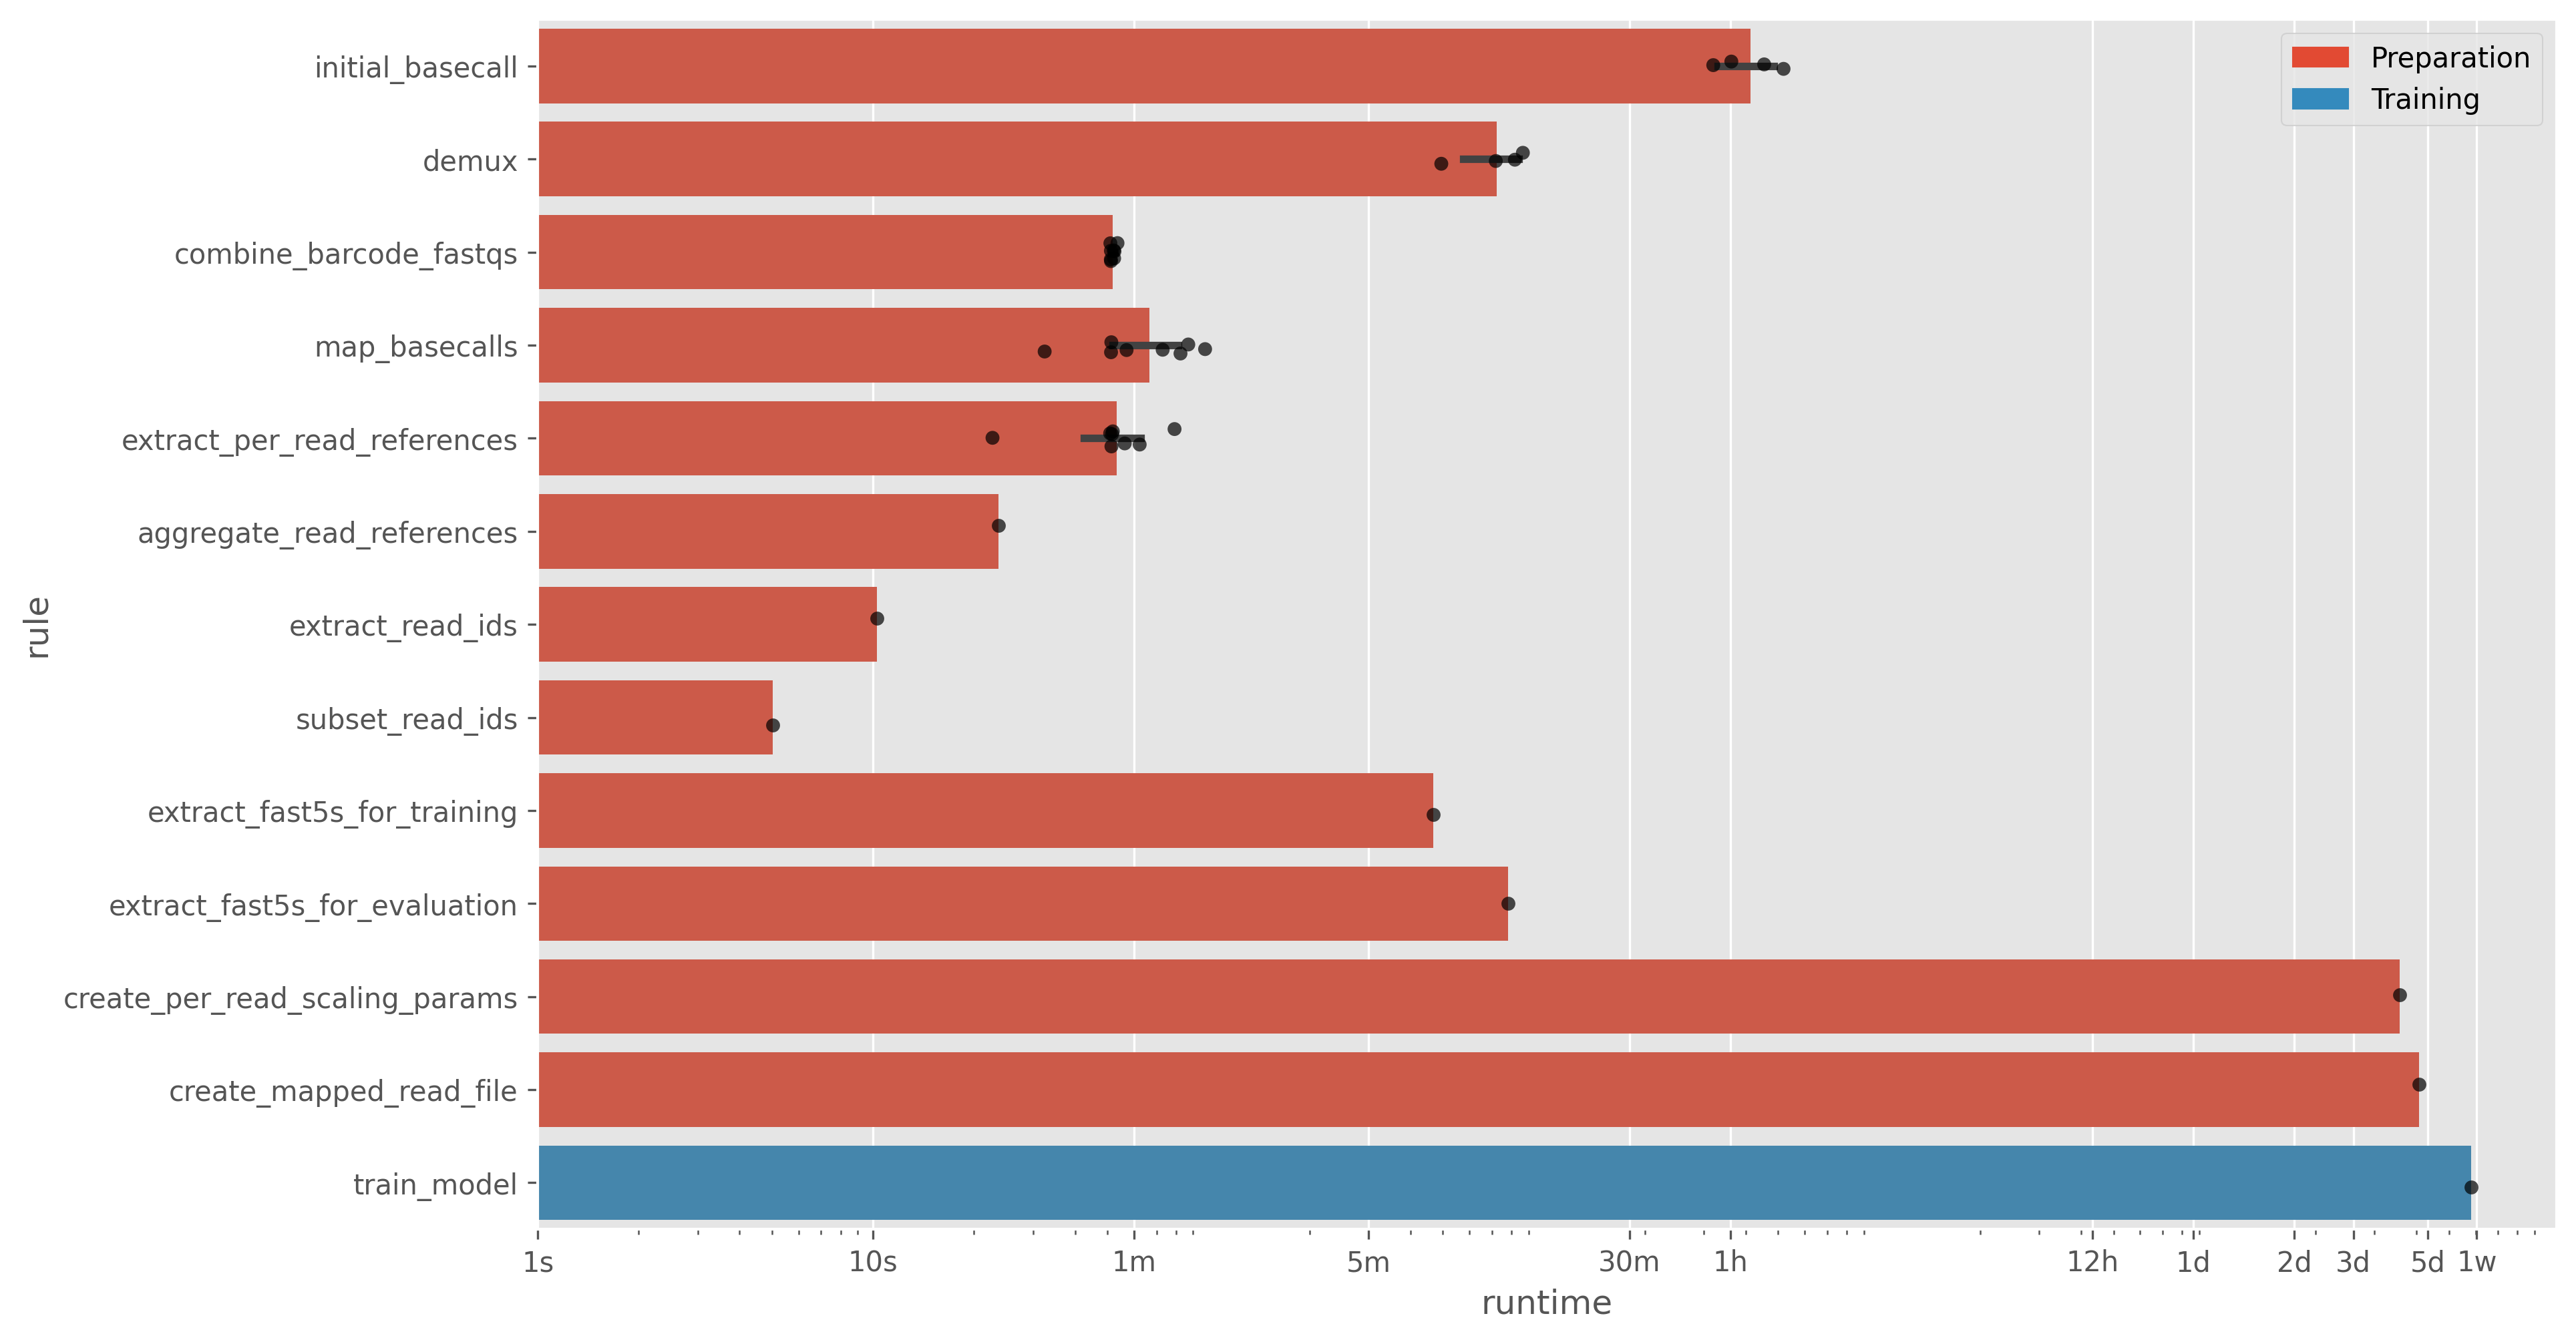
\includegraphics[width=0.9\textwidth]{Chapter4/Figs/prep_runtime.png}
\centering
\caption{Runtimes (x-axis) of the different stages (rules; y-axis) of preparing data for basecall model training. Each individual run is represented with a black point and rules that have multiple runs have black 95\% confidence interval bars. s=seconds; m=minutes; h=hours; d=days.}
\label{fig:prep_runtime}
\end{figure}

\autoref{fig:prep_runtime} shows the runtime of each step in the preparation phase of training. The two longest stages, trimming the raw signal (\vrb{create\_per\_read\_scaling\_params}) and mapping the raw signal to read-references (\vrb{create\_mapped\_read\_file}), took 4.1 and 4.7 days respectively. In total, the full preparation pipeline ran in 8.9 days. 

\subsubsection{Training}

The signal-to-sequencing mapping file produced from the preparation pipeline is the data file used for model training. In addition, we provide an initial model file from which training begins; the mLstm flipflop model distributed with \taiyaki{}.

We train the model using \taiyaki{}'s \vrb{train\_flipflop.py} script with the following parameters: a base layer size of 256; a model stride of 2; a window length over the data of 19; a minimum and maximum length of random training data chunks of 2000 and 4000, respectively; and a maximum learning rate of $0.002\sqrt{g}$, where $g$ is the number of GPUs used for training. The training took 162 hours (6.75 days) to complete on 2 GPUs and had a peak memory usage of 57GB. 

The final output from training the model is a checkpoint file, which we then convert to a \guppy{}-compatible JSON configuration file using \taiyaki{}.

%%%%%%%%%%%%%%%%%%%%%%%%%%%%%%%%%%%%%%%%%%%%%%%%%%%%%%%%%%%%%%%%%%%%%%%%%%%%%%%%%
\section{Evaluating a custom \ont{} basecalling model}

The model-training process produces a JSON file that can be used to basecall \ont{} reads with \guppy{}. The first step in evaluating whether our \mtb{}-specific model, 'tubby', provides improved accuracy compared to \guppy{}'s default model is to re-basecall (with tubby) the validation reads that were set aside prior to training. These validation reads provide an unbiased dataset to evaluate on as they were not involved in the training process. Our evaluation process closely mirrors that of Wick *et al.* who produced the first taxon-specific \ont{} basecalling model(CITE).  

We evaluate both the read- and consensus-level accuracy of reads produced by \guppy{} and tubby. For read-level accuracy, we map the basecalled data for each sample to the respective truth assembly and pool the read identities for each mapping over all samples. Our measure of read identity is the BLAST identity, defined as, for each alignment, the number of matching positions divided by the length of the alignment.  

To assess consensus-level accuracy, we first need to produce assemblies for each model's generated reads. To allow for comparison of these model-specific consensus sequences to the truth assembly, a reference-guided method is needed to ensure overall structure of the truth and consensus sequences is the same. We use `rebaler`(CITE), a tool developed for specifically this use-case. Briefly, `rebaler` aligns the reads to a reference sequence and replaces that sequence with the sequence from the best alignments, producing an unpolished assembly. After this, it polishes the assembly with `racon` to produce a consensus sequence. We then calculate the consensus accuracy by following a similar approach used for the read accuracy. However, as we have a single sequence, we cut the consensus into 10kbp chunks and treat these chunks as reads. These chunks are mapped to the reference/truth and the consensus accuracy is reported as the BLAST identity of the alignments produced.  

In addition to the read and consensus accuracy, we also evaluate the relative lengths of the reads/chunks in the alignment used for calculating the BLAST identity. The relative length is the length of the alignment, divided by the length of the read/chunk. This metric provides an indication of whether either model has a tendency towards deletions (relative length less than 1.0) or insertions (greater than 1.0).  

Lastly, we classify the the types of errors that occur in the assemblies produced from each model's output. The `rebaler` assembly for each model and sample combination was aligned to the sample's truth assembly using `nucmer`(CITE). `nucmer` produces all positions of difference - errors in this case - between the two sequences. We classify errors as Dcm if the reported difference occurs in a known 5-methylcystosine methyltransferases motif(CITE), homopolymer insertion or deletion if the difference involves as base being added/removed from a region containing 3 or more of that same base. All deletions, insertions, and substitutions that do not fit into one of these categories after reported in their own group.

%%%%%%%%%%%%%%%%%%%%%%%%%%%%%%%%%%%%%%%%%%%%%%%%%%%%%%%%%%%%%%%%%%%%%%%%%%%%%%%%%
\section{Read-level performance}

Read BLAST identity

The first evaluation metric, read BLAST identity, determines the read-level accuracy produced by the basecalling model. We align the basecalled reads to the truth assembly and calculate BLAST identity as, for each mapping, the number of matching bases divided by the length of the alignment. \autoref{fig:combined_basecall}A shows the tubby model has a higher read-level BLAST identity (median 0.941) than \guppy{} (median 0.920).

Relative read length

We define relative read length as the length of the aligned part of the read, divided by the total length of the read. The purpose of this metric is to see whether there is a bias towards insertions (greater than 1.0) or deletions (less than 1.0). \autoref{fig:combined_basecall}C shows that, at the read level, tubby has a slight tendency towards deletions (shorter reads) compared to \guppy{} with median relative read lengths of 0.982 and 0.993 respectively. However, this result is a little more complex than just looking at median values. The distribution of lengths for \guppy{} extends much further past 1.0 compared with tubby, indicating an increase in insertions. We will return to this result when we look at the error types.

% \begin{figure}
% 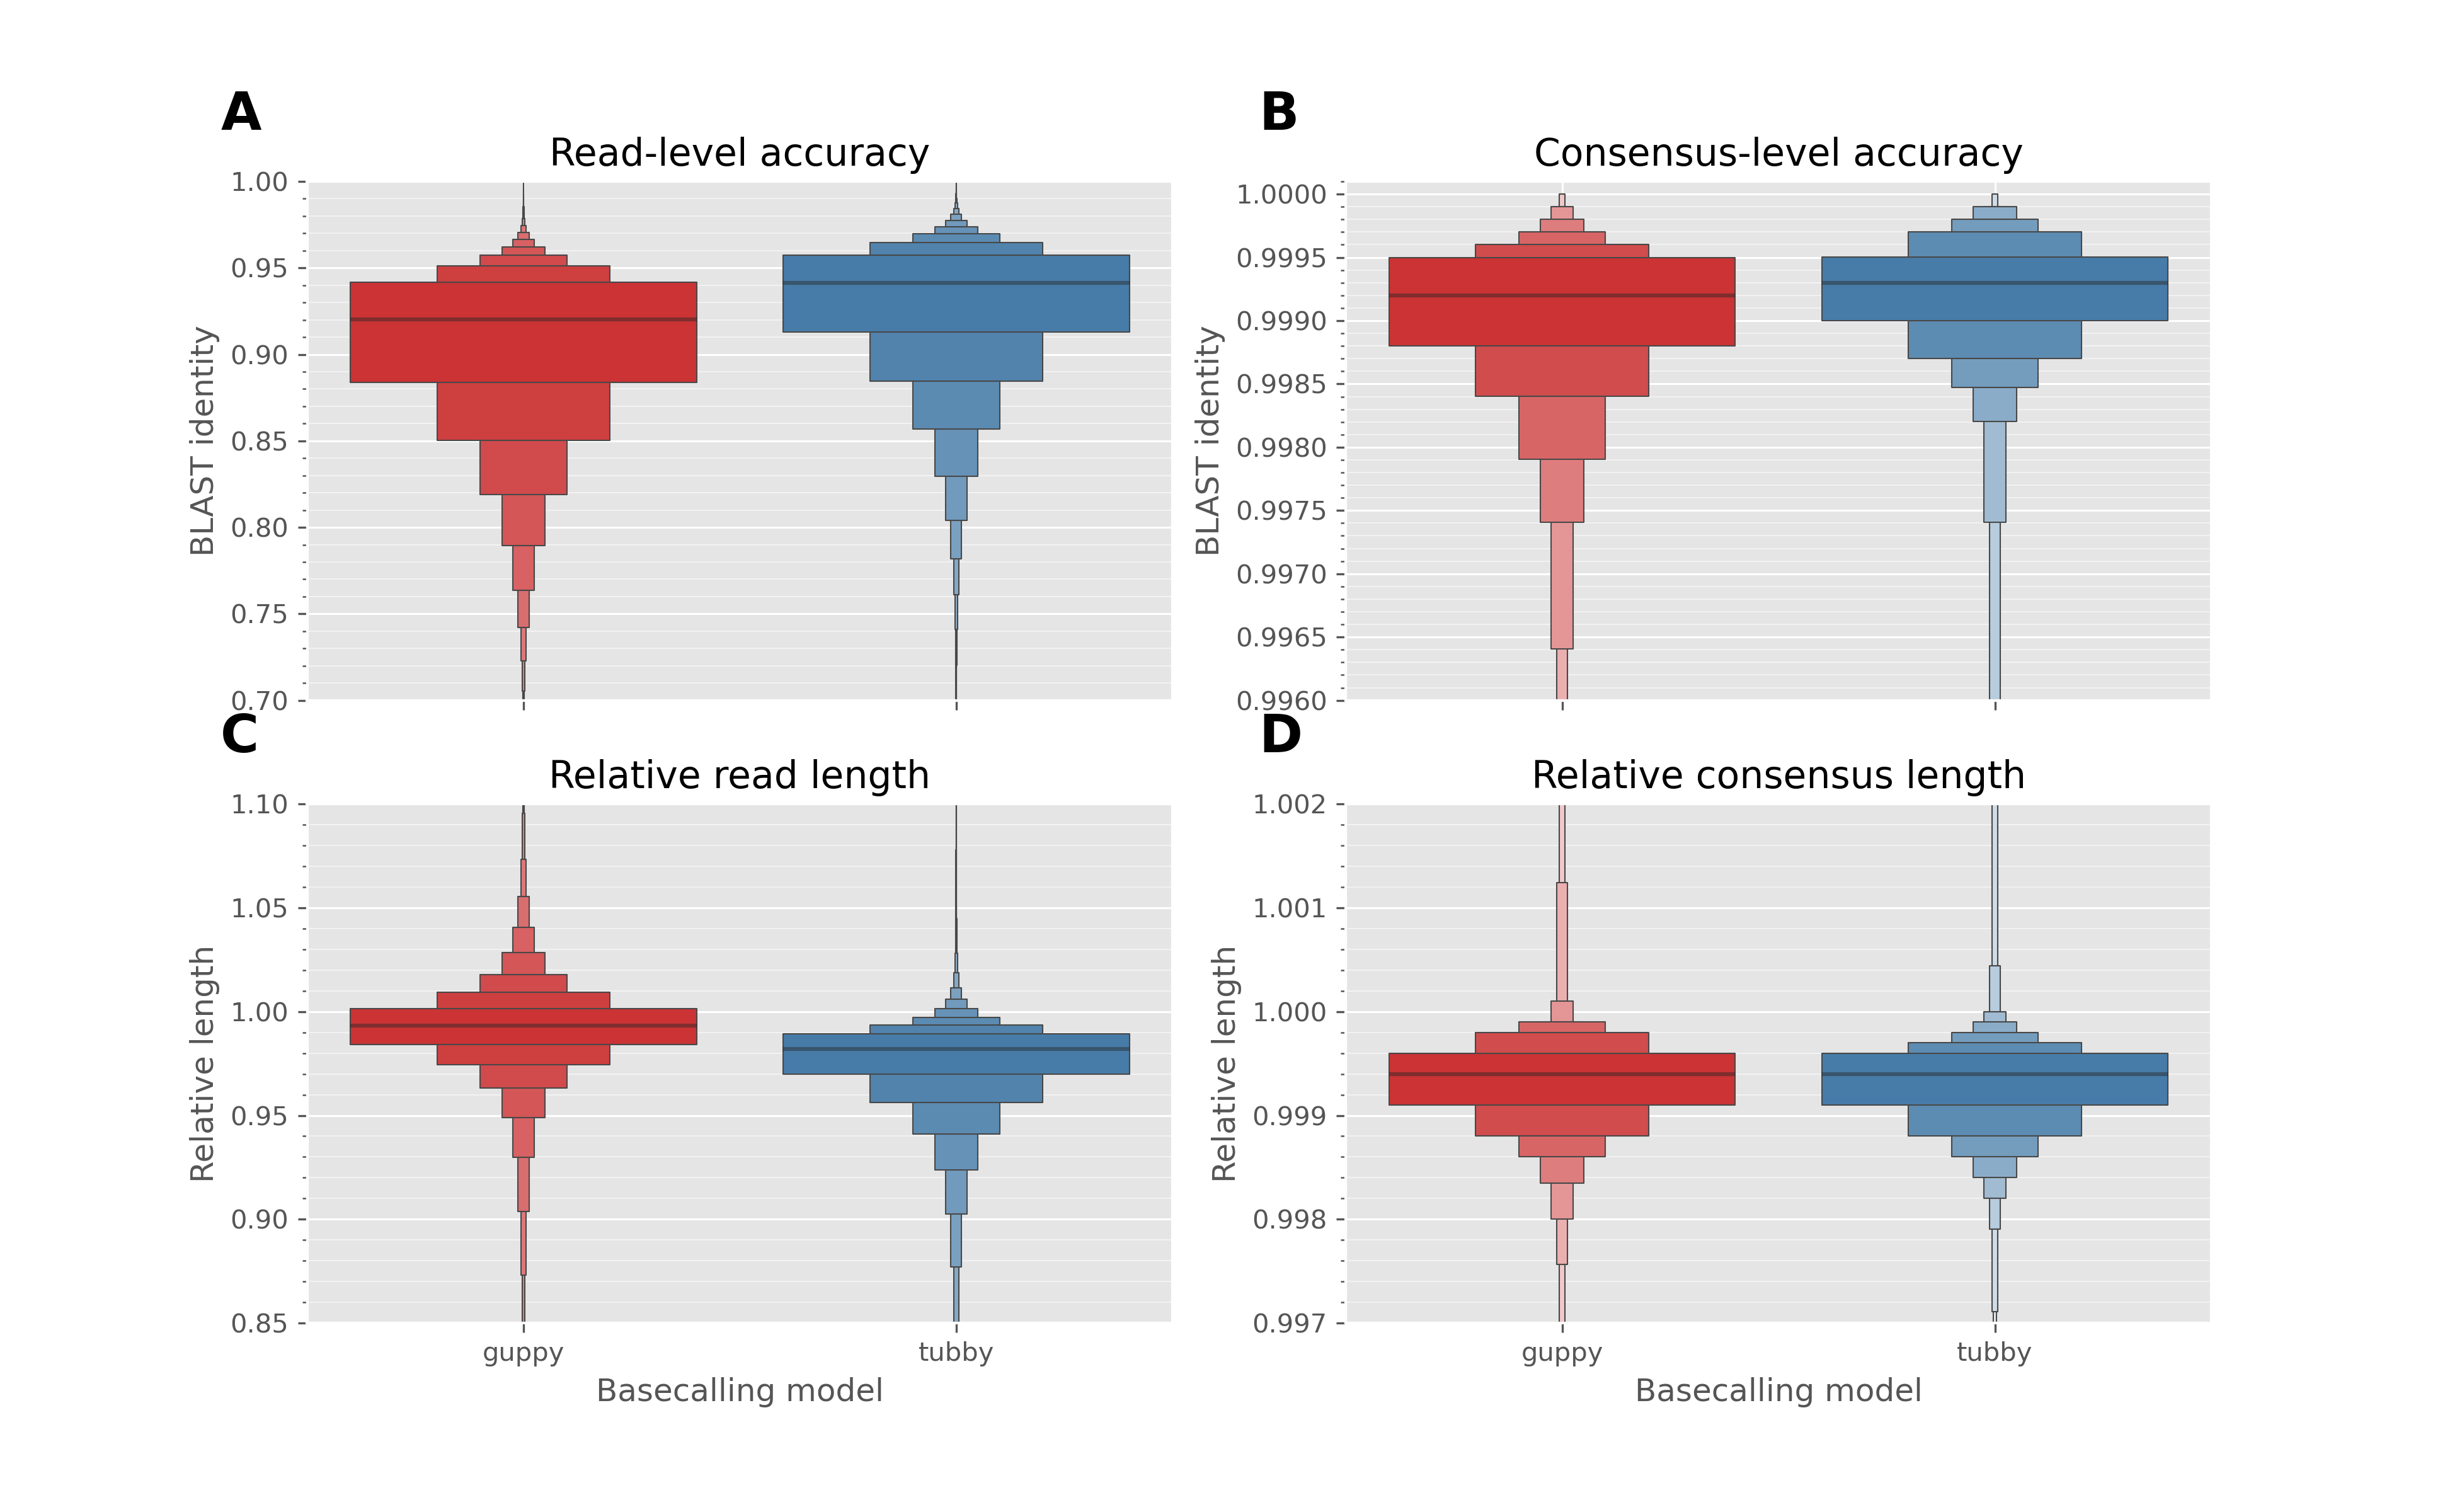
\includegraphics[width=1.0\textwidth]{Chapter4/Figs/combined_identity_relative_len.png}
% \centering
% \caption{A) Read BLAST identity (Y-axis) for the \mtb{}-specific basecalling model 'tubby' (blue) compared with the default \guppy{} model (red). BLAST identity is the number of matching bases (in a read alignment) divided by the length of the alignment. B) Consensus BLAST identity (Y-axis), where consensus refers to "chunks" of the genome assembly produced by the basecalled reads, for each model, mapped to the truth genome. C) Relative read length (Y-axis) for the two models. Relative read length is the length of the aligned part of the read, divided by the total length of the read. D) Consensus relative length. Relative length is the length of the aligned part of the consensus "chunk", divided by the total length of the "chunk". Note: the Y-axes have all been zoomed-in to allow closer inspection of the majority of data.}
% \label{fig:combined_basecall}
% \end{figure}

%%%%%%%%%%%%%%%%%%%%%%%%%%%%%%%%%%%%%%%%%%%%%%%%%%%%%%%%%%%%%%%%%%%%%%%%%%%%%%%%%
\section{Consensus-level performance}

To assess consensus accuracy the basecalled reads were assembled using `rebaler`. `rebaler` was developed by Wick *et al.* for the purposes of evaluating basecalling models and is a reference-guided assembly approach (see \todo{link to relevant methods section}). Here we show consensus accuracy in a similar manner to read identity. Each "read" in this context is the result of chopping the `rebaler` assembly of the reads up into 10kbp "chunks" to simulate reads. These chunks are then mapped back to the original assembly and we use BLAST identity as the measure of accuracy. \autoref{fig:combined_basecall}B shows tubby has higher consensus accuracy (median 0.9993) compared with \guppy{} (median 0.9992). The consensus accuracy improvement of 0.0001 equates to approximately 440 less erroneous positions in the \mtb{} assembly.

Error types

Here we classify the types of errors that occur in the `rebaler` assemblies and look at how these errors compare across models. To determine the errors, we categorise the differences between the truth and `rebaler` assemblies (see \todo{link to relevant methods}). \autoref{fig:error_types} shows that the greater part of the error types (for both models) are attributable to deletions, with most being homopolymer deletions. We do however see that, except for non-homopolymer deletions, tubby's errors are lower than \guppy{}'s \todo{add some concrete numbers}. In the case of both insertion types, tubby has approximately 3.5-fold less insertions than \guppy{} - although these constitute a small portion of the overall errors. Both models have a very low level of Dcm-methylation errors, which is a nice control of sorts as \mtb{} does not have any known 5-methylcystosine methyltransferases(CITE)\improvement{ensure the wording of this and correct and that the claim is also correct}.

% \begin{figure}
% 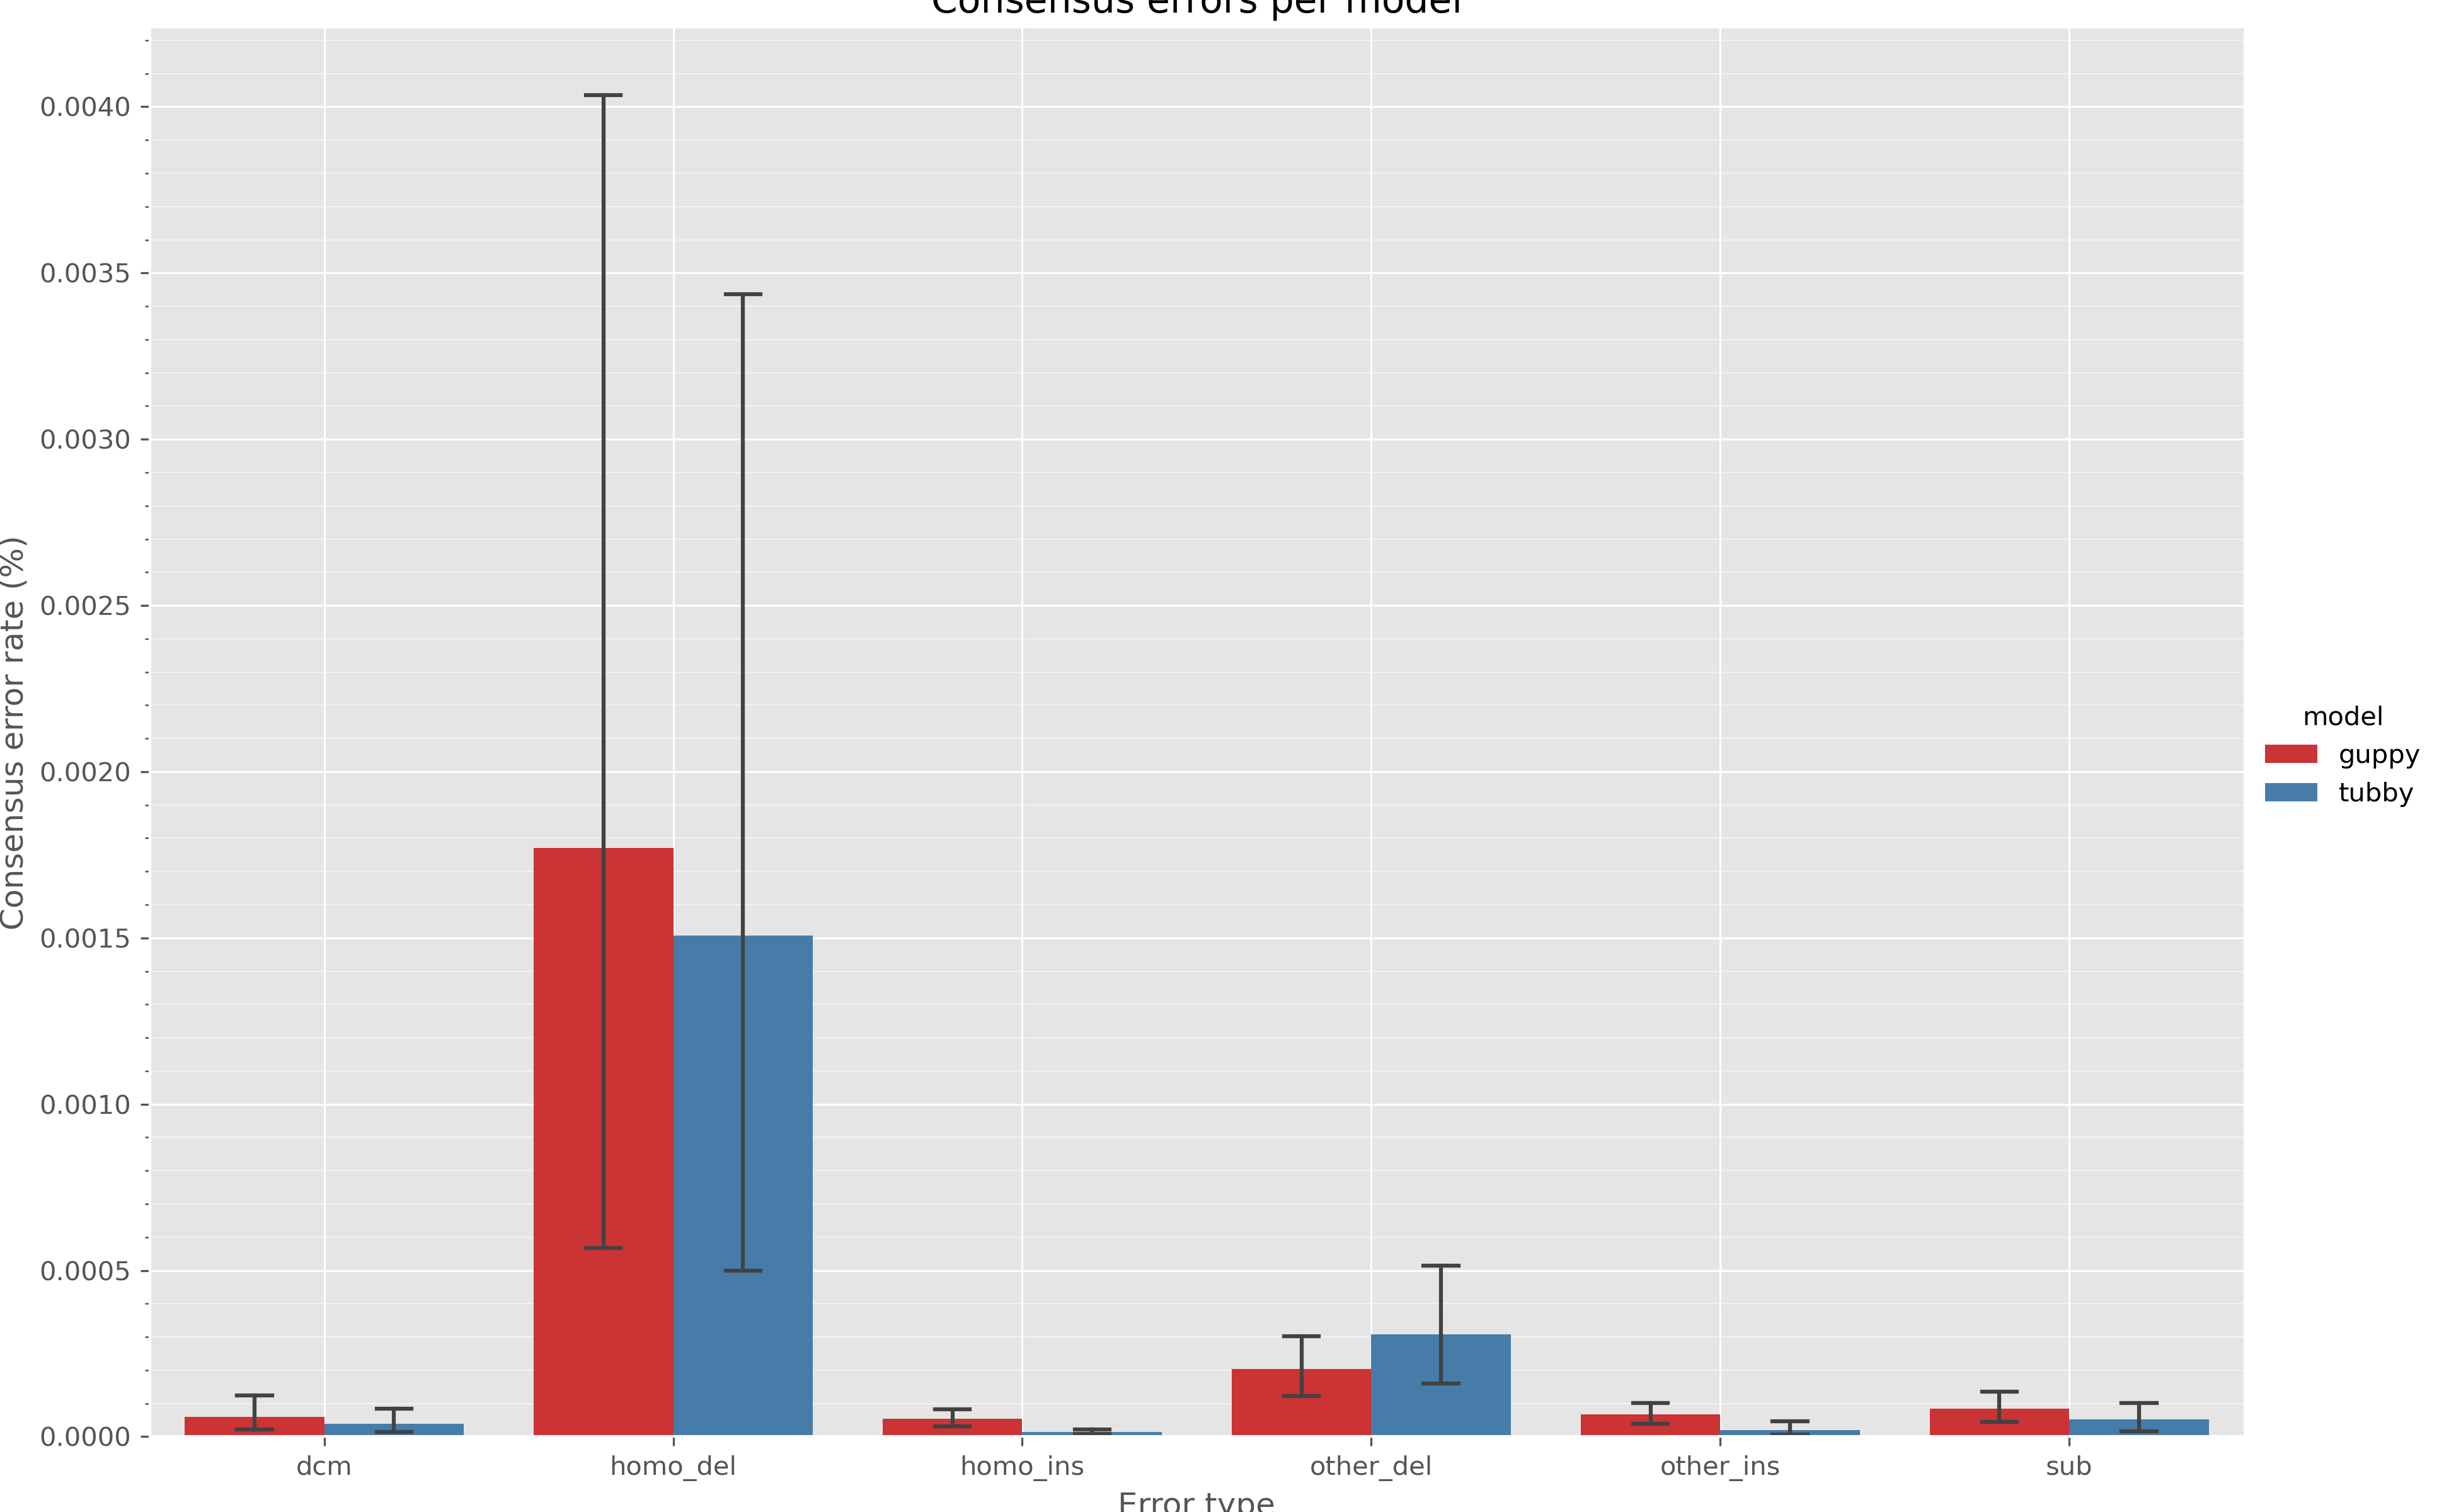
\includegraphics[width=1.0\textwidth]{Chapter4/Figs/consensus-error-types.png}
% \centering
% \caption{Error types in the `rebaler` assemblies produced from reads basecalled with tubby (blue) and \guppy{} (red). The consensus error rate is the percentage of the assembly these errors compose. The errors are per-assembly, so the confidence intervals represent variation in error types between samples/assemblies. dcm refers to Dcm-methylation motifs. homo\_ins/del are homopolymer insertions or deletions. sub is single-base substitutions.}
% \label{fig:error_types}
% \end{figure}

%%%%%%%%%%%%%%%%%%%%%%%%%%%%%%%%%%%%%%%%%%%%%%%%%%%%%%%%%%%%%%%%%%%%%%%%%%%%%%%%%
\section{Discussion}

%%%%%%%%%%%%%%%%%%%%%%%%%%%%%%%%%%%%%%%%%%%%%%%%%%%%%%%%%%%%%%%%%%%%%%%%%%%%%%%%%
\section{Conclusion}

%%%%%%%%%%%%%%%%%%%%%%%%%%%%%%%%%%%%%%%%%%%%%%%%%%%%%%%%%%%%%%%%%%%%%%%%%%%%%%%%%
\section{Future work}

%%%%%%%%%%%%%%%%%%%%%%%%%%%%%%%%%%%%%%%%%%%%%%%%%%%%%%%%%%%%%%%%%%%%%%%%%%%%%%%%%
\section{Availability of data and materials}